% LaTeX Template for report of CoastSat.Venice results
%Compile with LuaLaTex

%This document template was created with the assistance of ChatGPT for LaTeX scripting, table generation from CSV files, and figure handling

% Define the name of the site you want to report on and the sitename as defined without spaces
\newcommand{\sitename}{Caleta Olivia}
\newcommand{\folder}{Caleta_Olivia}

% These folder paths will auto compile
\newcommand{\csvTidesPath}{../Data/\folder/water_levels/FES2022_location_date_\folder.csv}
\newcommand{\csvWavesPath}{../Data/\folder/Waves/data/Virtual_Buoy.csv}
\newcommand{\csvSlopePath}{../Data/\expandafter\folder/slope_estimation}
\newcommand{\RunupPath}{../Data/\expandafter\folder/Runup}

% Citations should be in bibtex format and go in references.bib
\documentclass[a4paper, 11pt]{article}
\usepackage[top=3cm, bottom=3cm, left = 2cm, right = 2cm]{geometry} 
\geometry{a4paper} 
\usepackage[utf8]{inputenc}
\usepackage{textcomp}
\usepackage{graphicx} 
\usepackage{amsmath,amssymb}  
\usepackage{bm}  
\usepackage{csvsimple}
\usepackage{memhfixc}
\usepackage{pdfsync}  
\usepackage{fancyhdr}
\pagestyle{fancy}
\usepackage{pgfplots}  % Needed for rounding numbers
\usepackage{hyperref}

%references
\usepackage{natbib}
\bibliographystyle{chicago}


\title{\sitename - Wave Runup Report}
%\date{}

\begin{document}
\maketitle

This report is compiled with the results of the CoastSat.Venice tool for the calculation of runup values for paleo sea-level applications \citep{alessio_rovere_2024_14543991}, available at \href{https://doi.org/10.5281/zenodo.14543991}{this link}. The tool is based upon the work of \cite{Coastsat,Coastsat_slope} for the slope extraction from satellite data, on the runup models implemented in \cite{chris_leaman_2020_3629949} and on the tidal and wave models shown below. For a case study, see 

\section*{Water levels}
Water level data were extracted at the coordinates and over the period shown in \autoref{tab:water_level_data} using the FES2022 global tidal model \citep{carrere2022new} at a point slightly offshore of \sitename.

\begin{table}[ht]
    \centering
    \csvreader[
        head to column names,
        before reading={\catcode`\#=12}, % Handle special characters
        tabular=|l|l|,                  % 2-column table (key-value)
        table head=\hline Property & Value \\ \hline,
        late after line=\\ \hline
    ]{\csvTidesPath}{}                       % CSV Path
    {Latitude & \pgfmathprintnumber[precision=6]{\csvcoli} \\ 
    Longitude & \pgfmathprintnumber[precision=6]{\csvcolii} \\ 
    Start date-time & \csvcoliii \\ 
    Start date-time & \csvcoliv}
    \caption{Location of water level extraction point and dates of water level extraction for \sitename.}
    \label{tab:water_level_data}
\end{table}

\begin{figure}[ht]
    \centering
	\includegraphics[width=\textwidth]{../Data/\expandafter\folder/water_levels/\expandafter\folder_tide_timeseries.jpg}
    \caption{Water levels extracxted from the FES22 tidal model for \sitename. Left: water level time series. Right: Histogram of water level data. Blue dashed line represents mean tidal level (MTL).}
	\label{fig:tide_timeseries}
\end{figure}

\pagebreak

\section*{Wave data}
Wave data is retrieved from the Copernicus Marine Environment Monitoring Service (CMEMS) WAVeReanalYSis \citep[WAVERYS,][]{law2021waverys}. WAVERYS takes into account oceanic currents from the GLORYS12 physical ocean reanalysis \citep{lellouche2018recent} and assimilates wave heights from altimetry missions and  directional wave spectra from Sentinel 1 synthetic aperture radar from 2017 onwards. This dataset spans the last \textasciitilde43 years (01 Jan 1980 to 30 Sept 2023). The wave data was sampled at a virtual buoy slightly offshore \sitename \autoref{tab:virtual_buoy}, and the average wave height, period and direction is shown in \autoref{fig:waves_average}.

\begin{table}[ht]
    \centering
    \csvreader[
        head to column names,
        before reading={\catcode`\#=12},  % Handle special characters
        tabular=|l|l|,                    % Two columns (Label | Value)
        table head=\hline Property & Value \\ \hline,  % Header with two columns
        late after line=\\ \hline
    ]{\csvWavesPath}{}{
        Latitude & \pgfmathprintnumber[precision=6]{\csvcoli} \\  % First row
        Longitude & \pgfmathprintnumber[precision=6]{\csvcolii}   % Second row
    }
    \caption{Coordinates of water level extraction point for \sitename.}
    \label{tab:virtual_buoy}
\end{table}


\begin{figure}[ht]
    \centering
	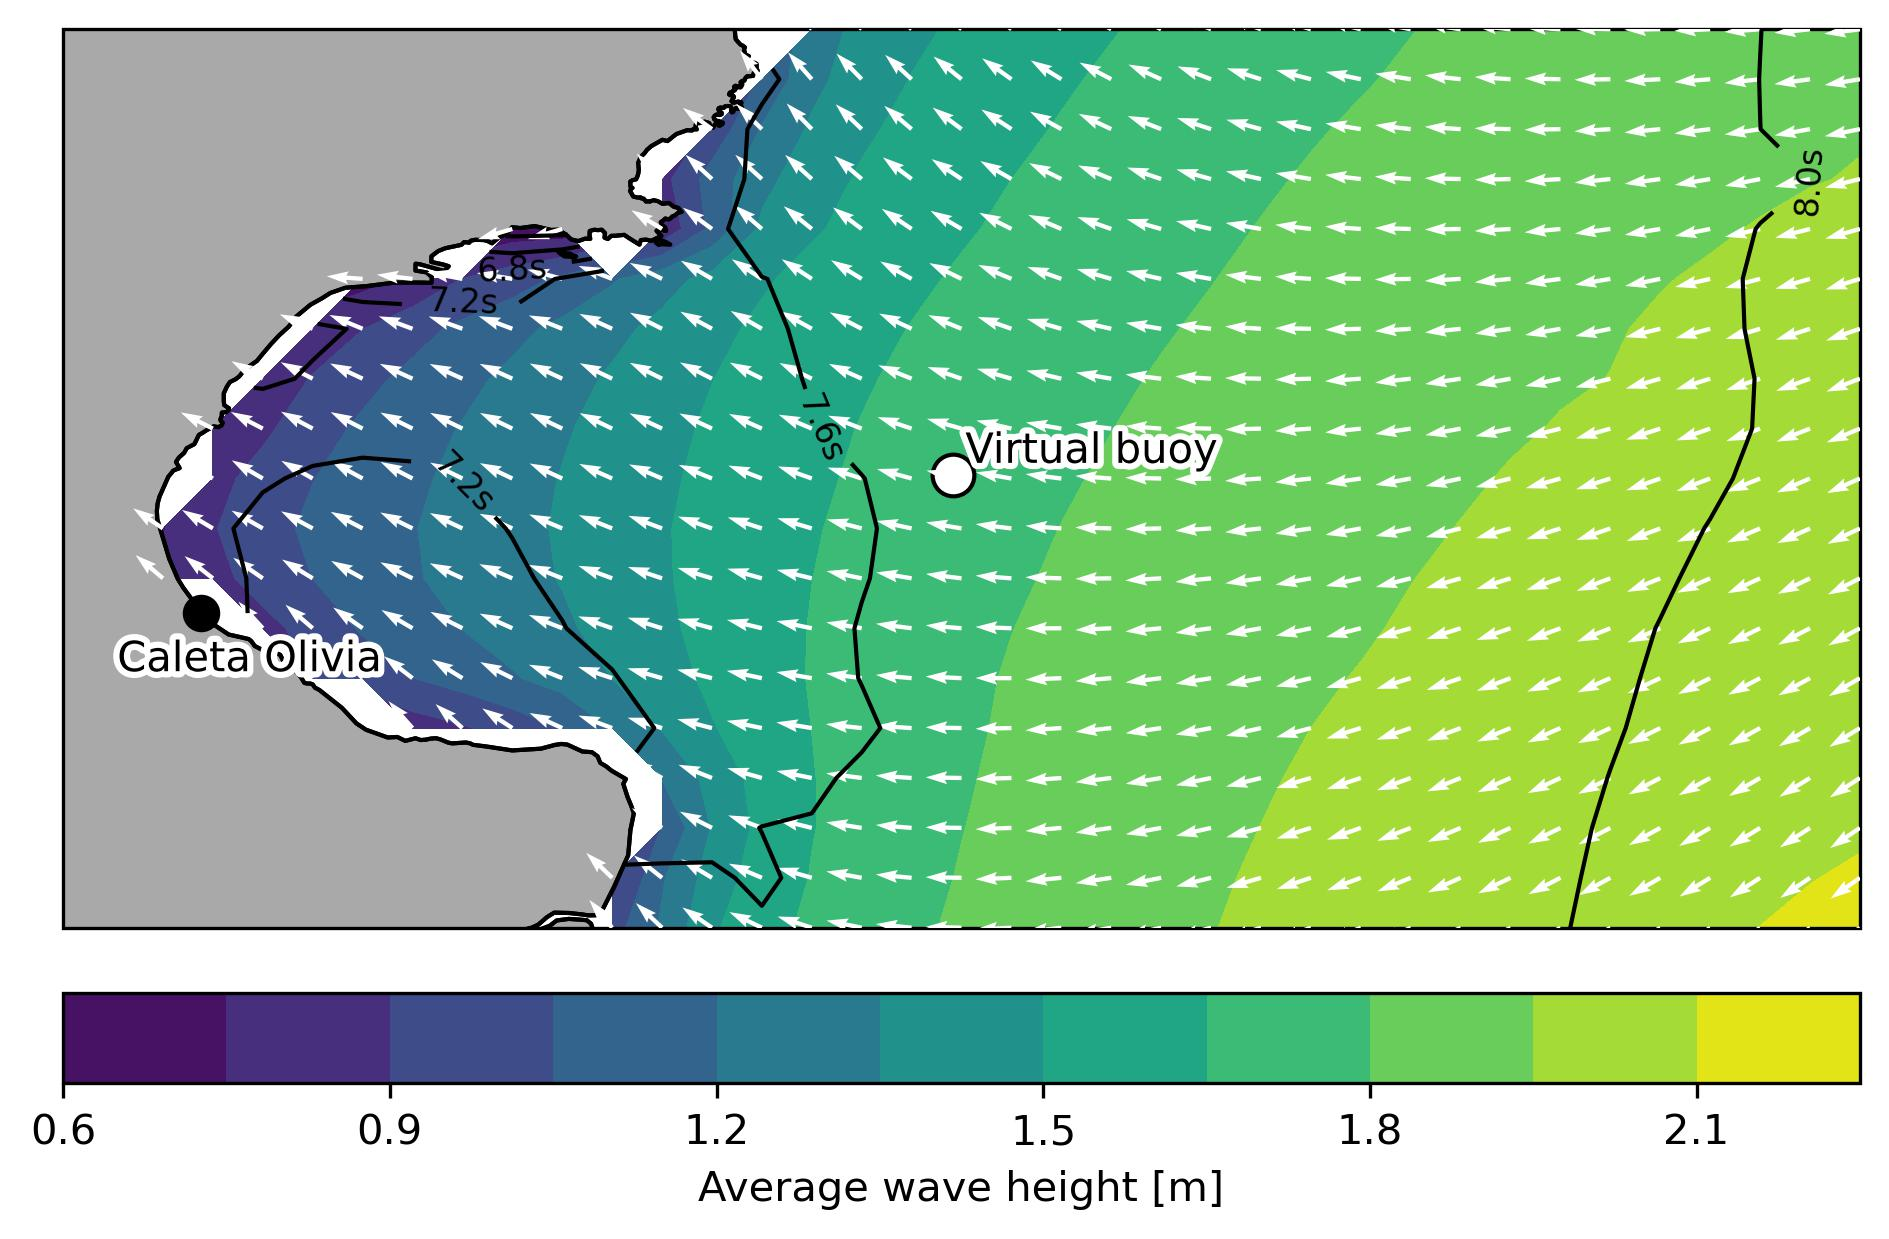
\includegraphics[width=\textwidth]{../Data/\expandafter\folder/Waves/img/Wave_height_direction_period_map.jpg}
    \caption{Average wave height (colored countours), period (black line with labels) and direction (arrows) extracted for the area of interest from the WAVERYS data. In the figure are shown the location of the virtual buoy (coordinates in \autoref{tab:virtual_buoy}) and the location of the site of interest.}
	\label{fig:waves_average}
\end{figure}

\pagebreak
The wave data at the virtual buoy was culled to include only the waves directed perpendicularly to the shore (\autoref{fig:waves_histograms}, right panels). Those are the data used to calculate the runup on the coast. The wave rose is shown in \autoref{fig:combined_figure}.

\begin{figure}[ht]
    \centering
	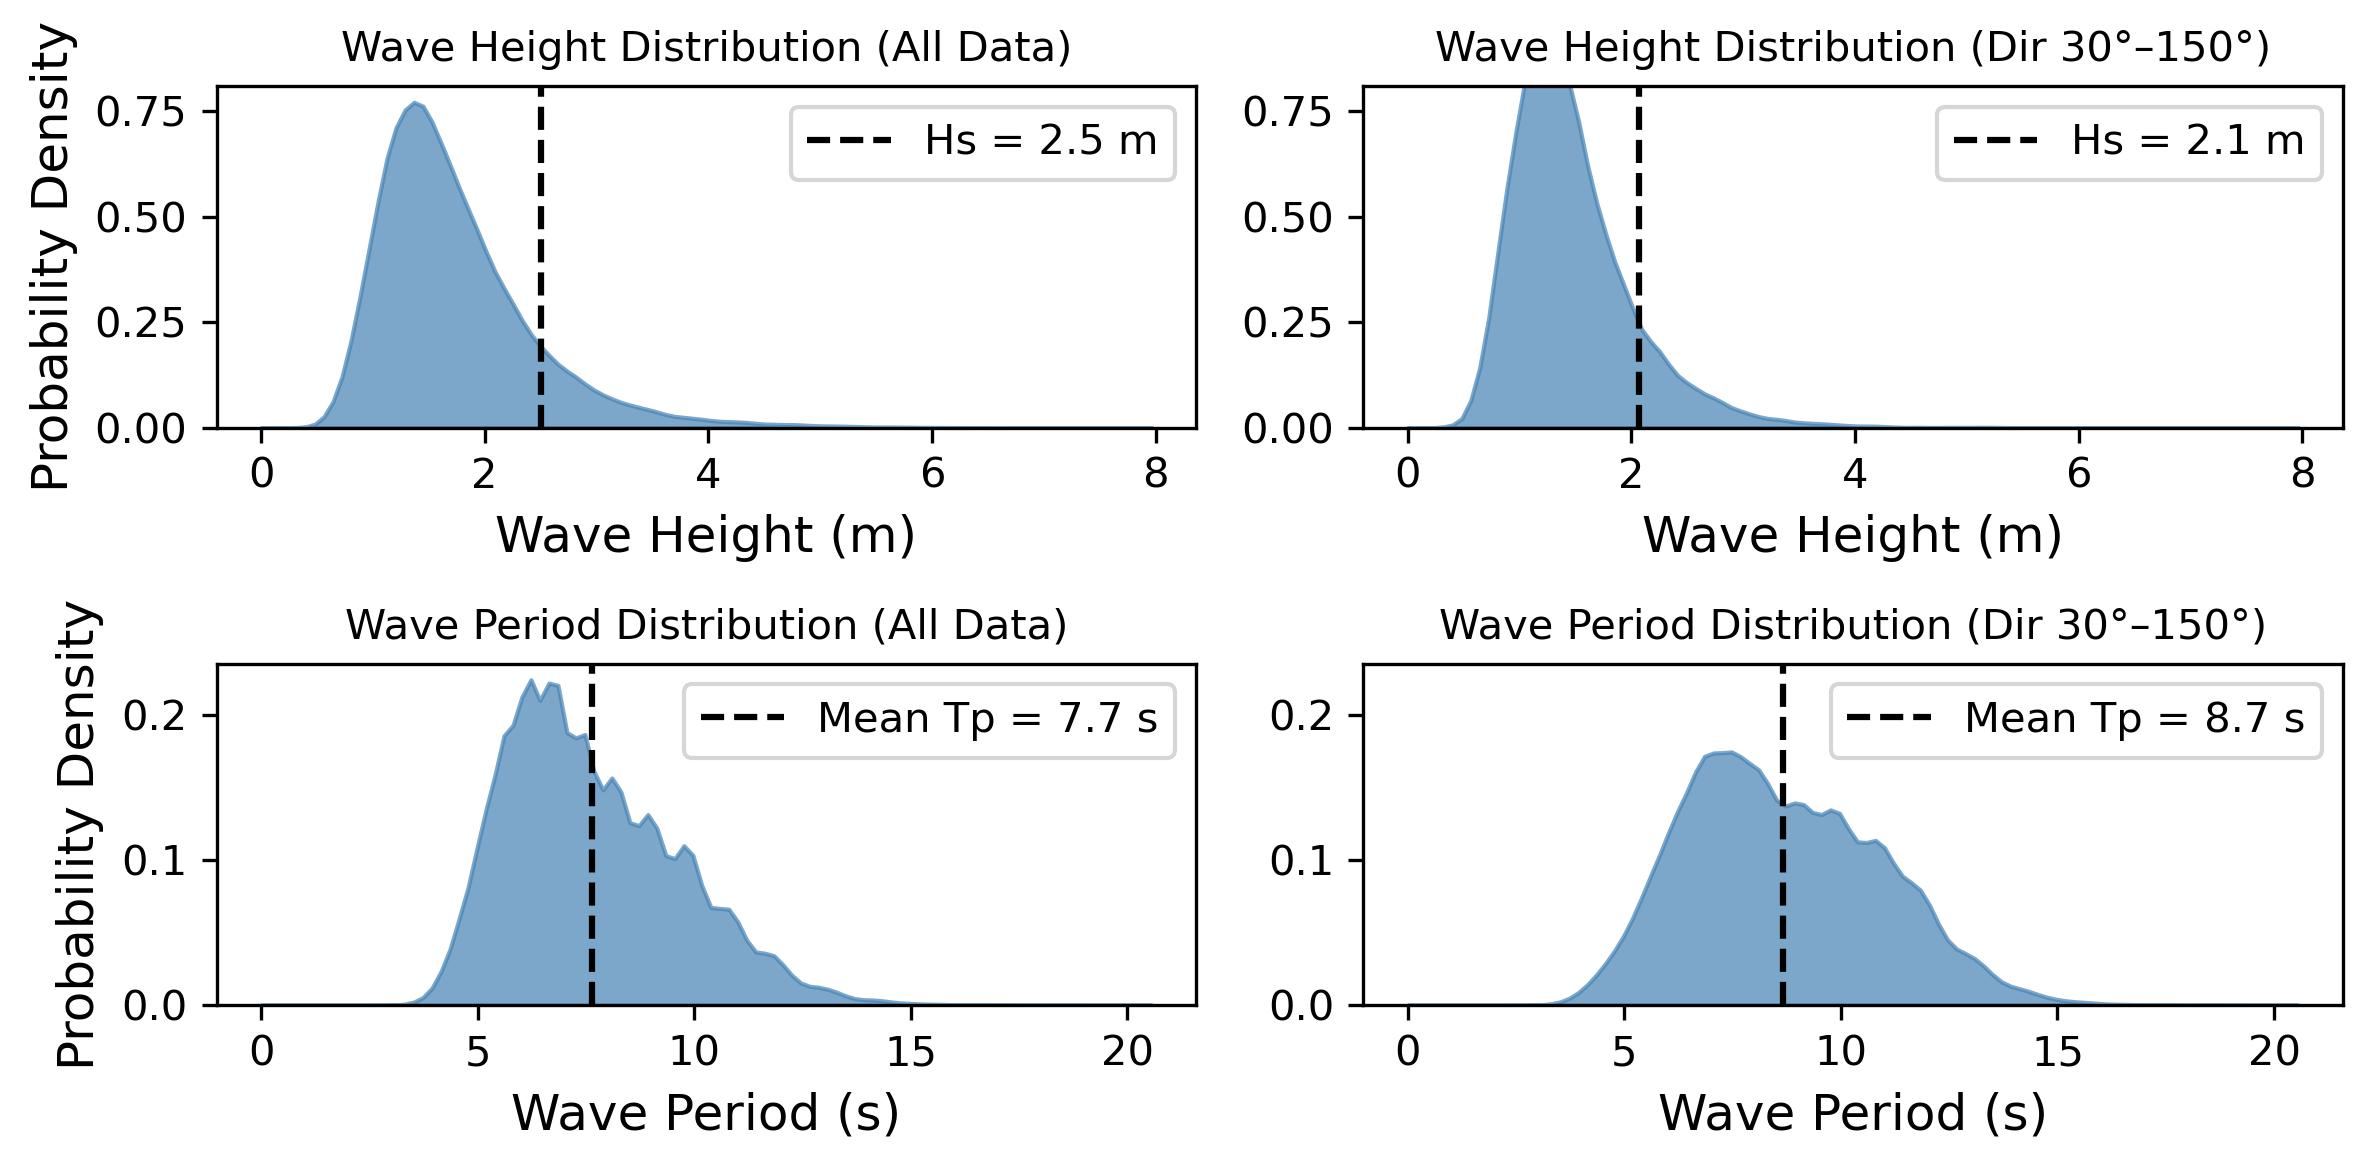
\includegraphics[width=0.7\textwidth]{../Data/\expandafter\folder/Waves/img/Wave_Height_and_Period_KDE_Filtered_Filled.jpg}
    \caption{Left panels: probability distribution of wave height (upper) and period (lower) for all the wave directions in the study area. Right panels: the same are left panels, but only for the directions more perpendicular to the coast.}
	\label{fig:waves_histograms}
\end{figure}

\begin{figure}[htb]
    \centering
    \begin{minipage}{0.48\textwidth}
        \centering
        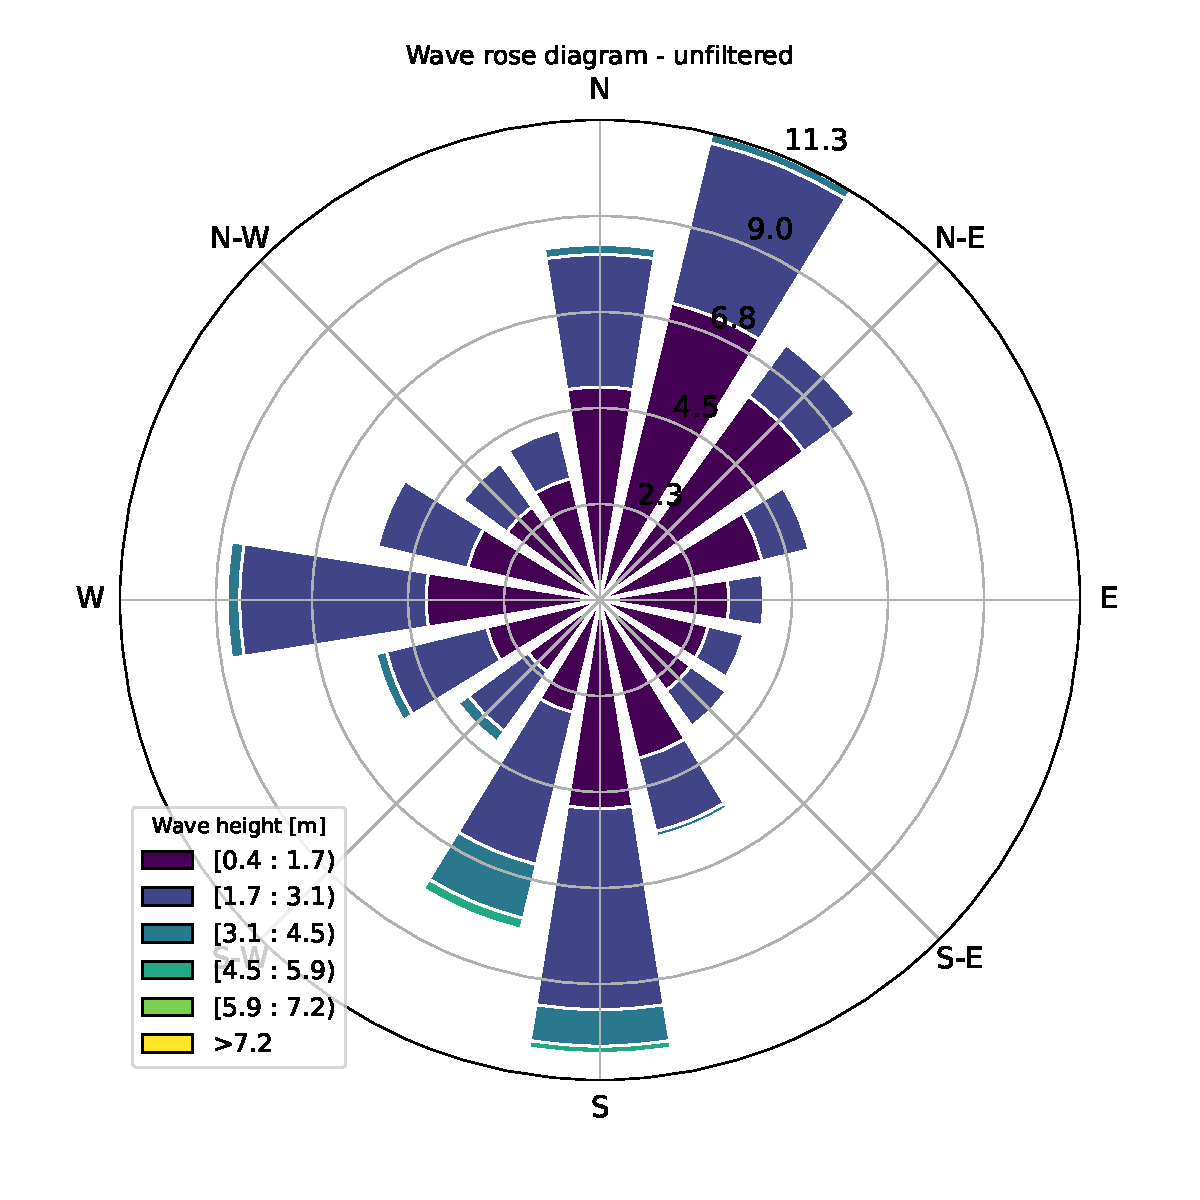
\includegraphics[width=\textwidth]{../Data/\expandafter\folder/Waves/img/Windrose_HS_unfiltered.pdf}
        \label{fig:panel1}
    \end{minipage}
    \hfill
    \begin{minipage}{0.48\textwidth}
        \centering
        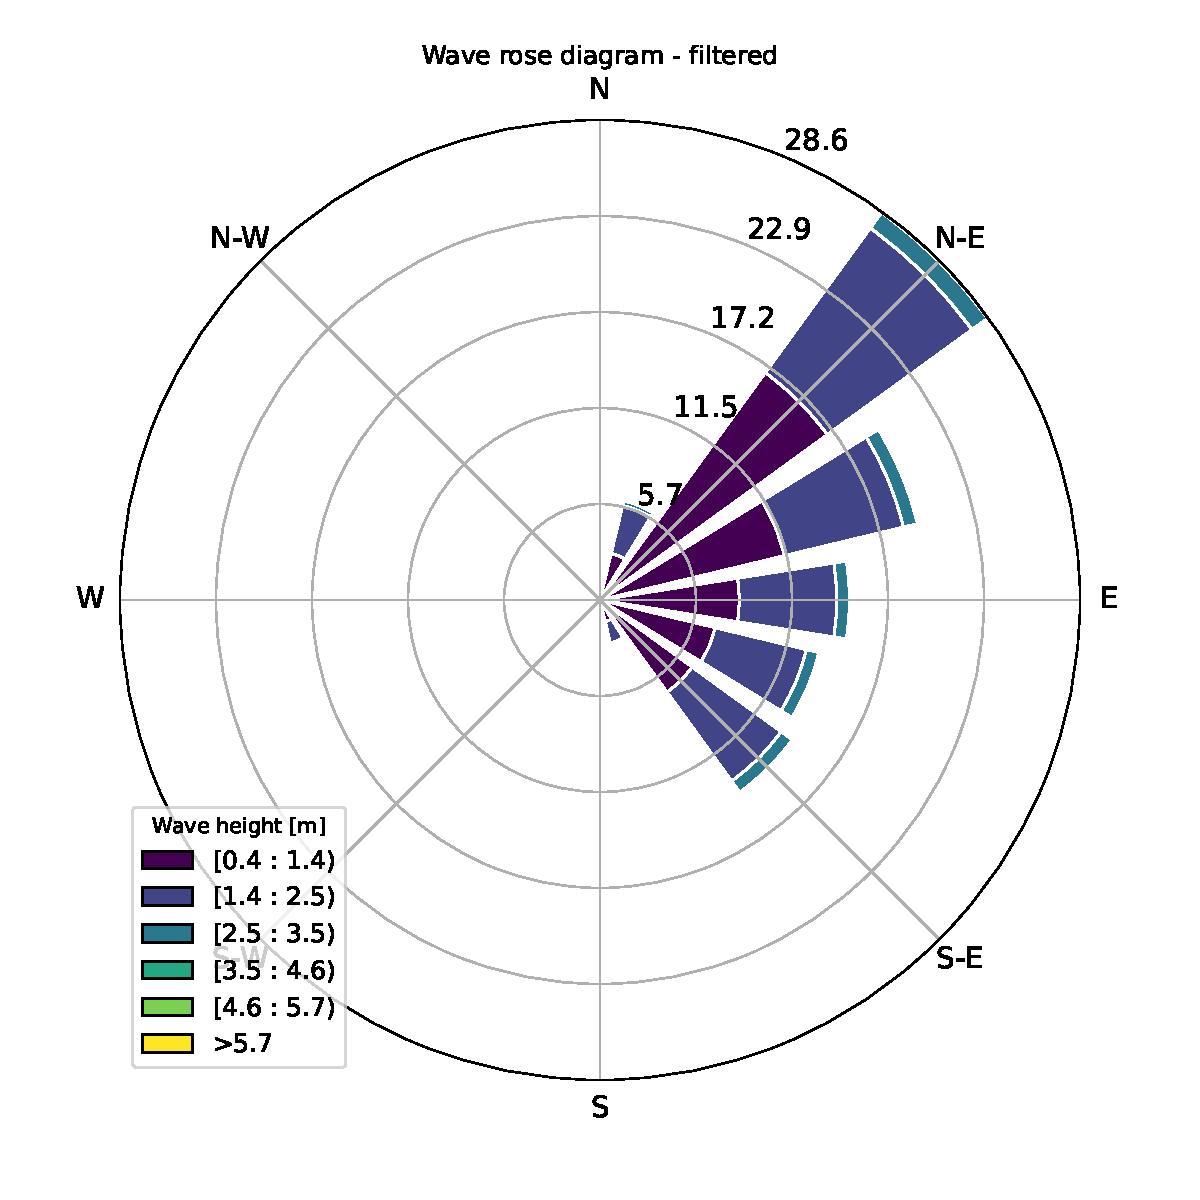
\includegraphics[width=\textwidth]{../Data/\expandafter\folder/Waves/img/Windrose_HS_filtered.pdf}
        \label{fig:panel2}
    \end{minipage}
    \caption{Left: wave rose, unfiltered for wave direction, at the virtual buoy. Right: same, filtered for shore-perpendicular wave directions.}
    \label{fig:combined_figure}
\end{figure}

\pagebreak
\section*{Beach slope}

\input{\expandafter\csvSlopePath/slope_method.txt}, shown in \autoref{tab:slope_data}. The slope was sampled within the confidence intervals with a random triangular sampling as shown in \autoref{fig:slope_image}.

\begin{table}[ht]
    \centering
    \csvreader[
        head to column names,              % Use first row as header
        before reading={\catcode`\#=12},   % Handle special characters
        tabular=|c|c|c|c|,                 % 4 columns centered
        table head=\hline Transect \# & CI Lower (5\%) & CI Upper (95\%) & Slope Average \\ \hline,
        late after line=\\ \hline
    ]{\csvSlopePath/Transects_slope.csv}{} % Corrected path
    {\csvcoli & \csvcolii & \csvcoliii & \pgfmathprintnumber[fixed,precision=3]{\csvcoliv}}
    \caption{Beach slope and confidence intervals for each beach transect at the site of interest.}
    \label{tab:slope_data}
\end{table}


\begin{figure}[ht]
    \centering
	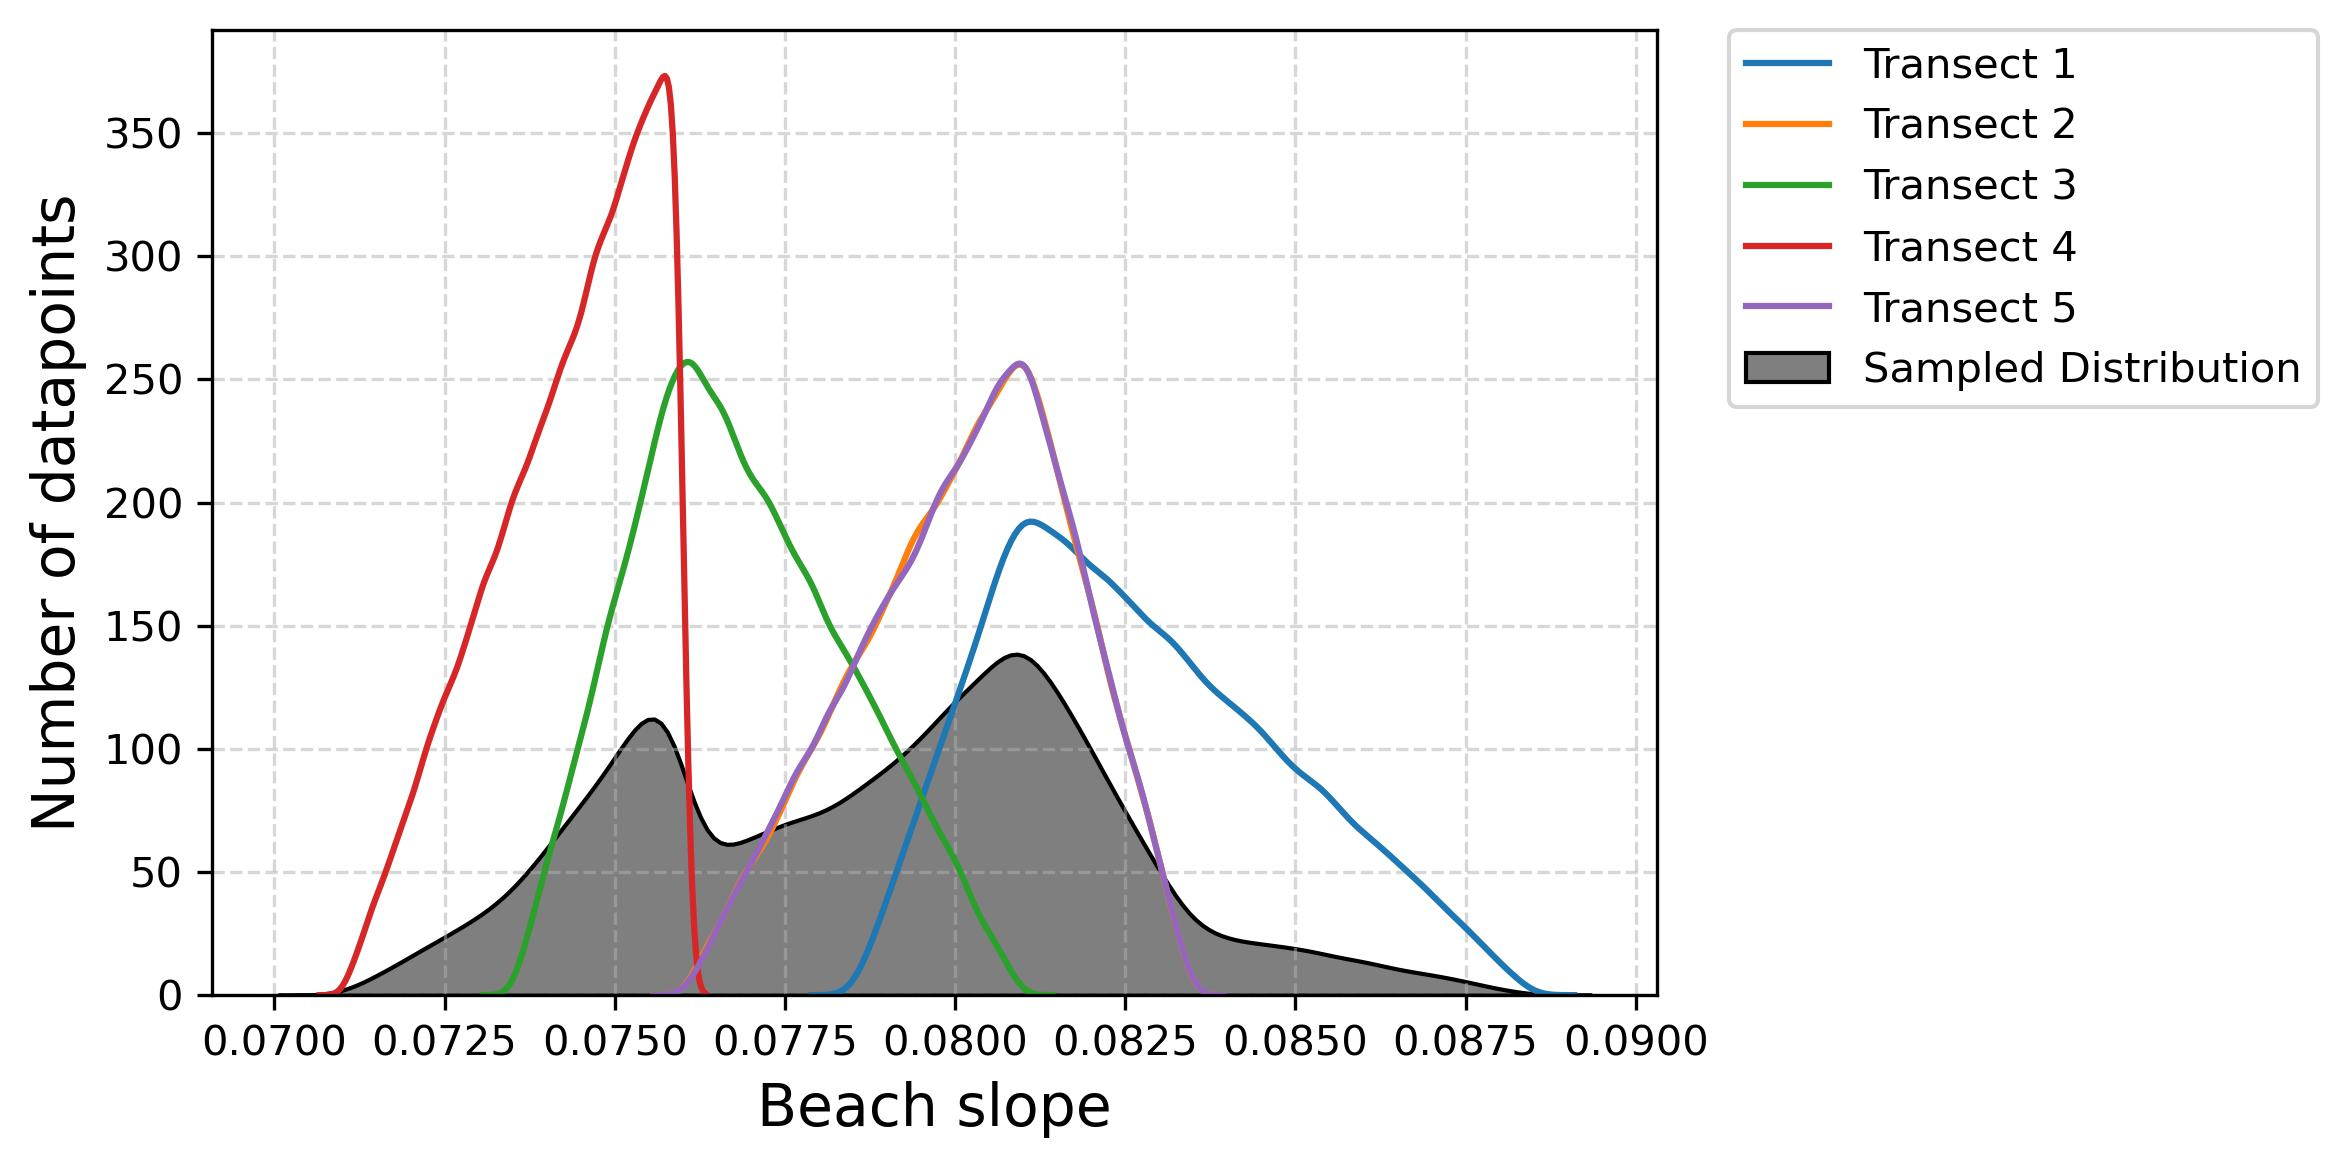
\includegraphics[width=\textwidth]{\expandafter\RunupPath/img/Slope_sampling.jpg}
    \caption{Slope distribution used in runup calculations (gray area) and slope of each single transect (colored lines).}
	\label{fig:slope_image}
\end{figure}

\pagebreak
\section*{Runup calculations}
The runup is calculated for the modern wave conditions with nine different models \citep{STOCKDON2006573,vousdoukas2012coastal,HOLMAN1986527,POWER201947,passarella2018use,senechal2011wave,ATKINSON201715,ruggiero2001wave,nielsen2009coastal}. These are shown separately in \autoref{fig:runup_modern}.

\begin{figure}[ht]
    \centering
	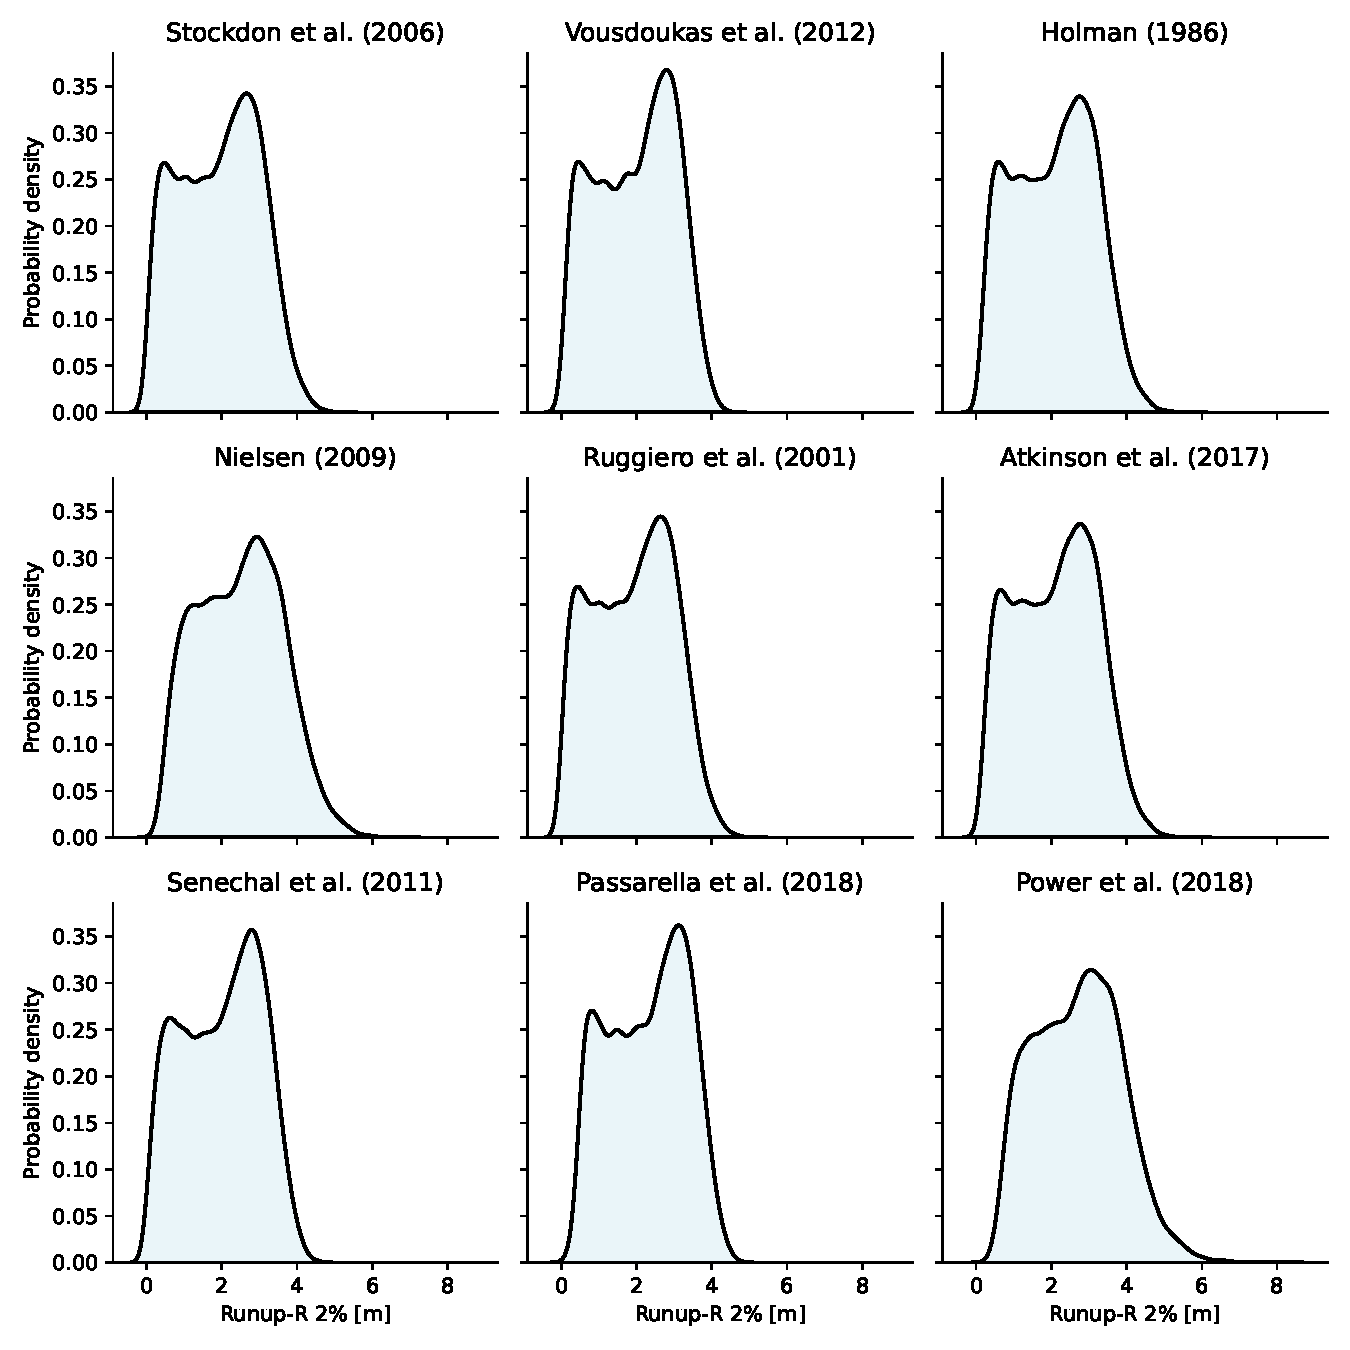
\includegraphics[width=\textwidth]{\expandafter\RunupPath/img/runup_modern_all.pdf}
    \caption{Modern runup calculated using nine empyrical models combined with wave and tide data atthe site of interest.}
	\label{fig:runup_modern}
\end{figure}

\pagebreak
The runup over longer time period (synthetic runup) is shown in \autoref{fig:runup_all}, alongside with the cumulative modern runup derived merging the probability distributions shown in \autoref{fig:runup_modern}.

\begin{figure}[ht]
    \centering
	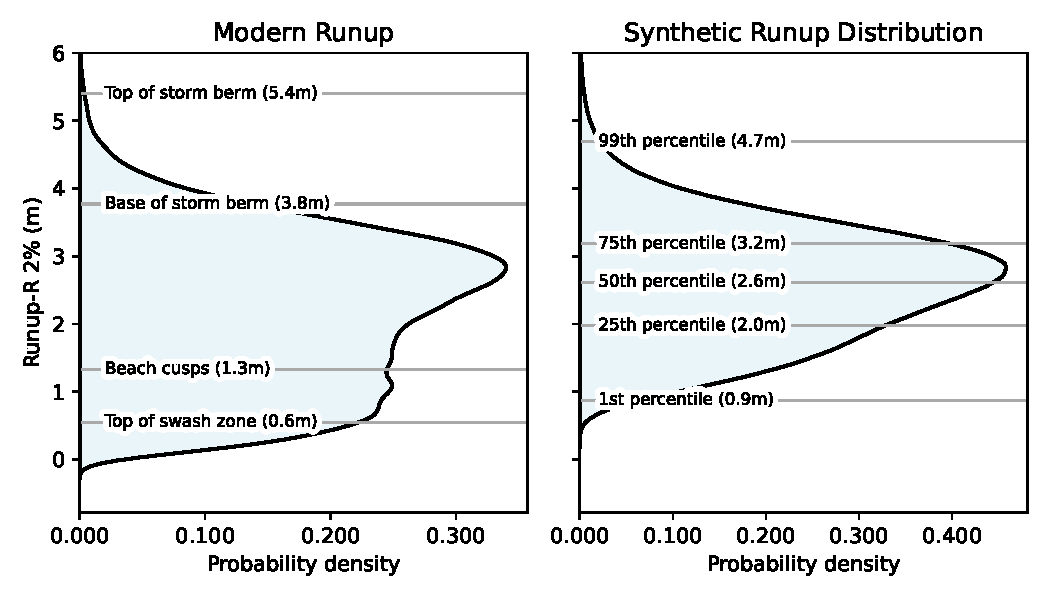
\includegraphics[width=\textwidth]{\expandafter\RunupPath/img/two_panel_runup.pdf}
    \caption{A) Probability density plots representing simulated 2\% wave runup (R2) at \sitename between 1980 and 2024, for waves with directions between NNE and SSE and reaching the coast in tidal conditions from MSL to high tide. Elements measured on the modern shoreline (if present) are plotted as grey lines with labels. Right) Probability density plot representing simulated 2\% wave runup at \sitename for the synthetic dataset, calculated as described in the main text. The grey lines show the 1st, 25th, 50th, 75th and 99th percentiles of this distribution.}
	\label{fig:runup_all}
\end{figure}

\pagebreak

\bibliography{references}
\end{document}